\documentclass{article}
\usepackage{graphicx}
\begin{document}
\section*{String manipulation in action}
Let's face it. Surveying literature is boring. That's why your guide makes 
\emph{you} do it. It's easy to make Python do it for you instead. You don't even
have to feel bad about it -- Python has no feelings! Unless, of course:
\begin{figure}[h]
\begin{center}
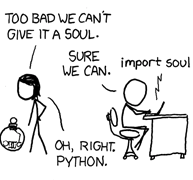
\includegraphics[width=100pt]{../../pictures/import_soul.png}
\end{center}
\end{figure}
\newline \texttt{docs} has a collection of documents related to programming
history and programming practices. Yawn. Your guide has asked you to work
with Python for this project, and you don't want to waste your time sifting through
irrelevant literature. You can write a program that:
\begin{enumerate}
\item Counts the number of times the word `Python' appears in a document (if at all)
\item Sorts documents by the frequency of occurrence
\end {enumerate}
Silly as this example may seem, you can easily imagine that even a slightly
more complex program can save you a lot of time, sweat and tears.
\subsection*{Useful tips:}
\begin{itemize}
\item To convert a pdf to a text file, use the shell command \texttt{pdftotext foo.pdf}
\item To conver \emph{all} pdfs to text files, do:
\begin{verbatim}

for file in *.pdf
do
pdftotext $file
done

\end{verbatim}

\item Pass text files to Python as command-line arguments.
\item See \texttt{f.read() and str.split()}
\end{itemize}
\end{document}
